\begin{figure}[htbp]
 \begin{center}
  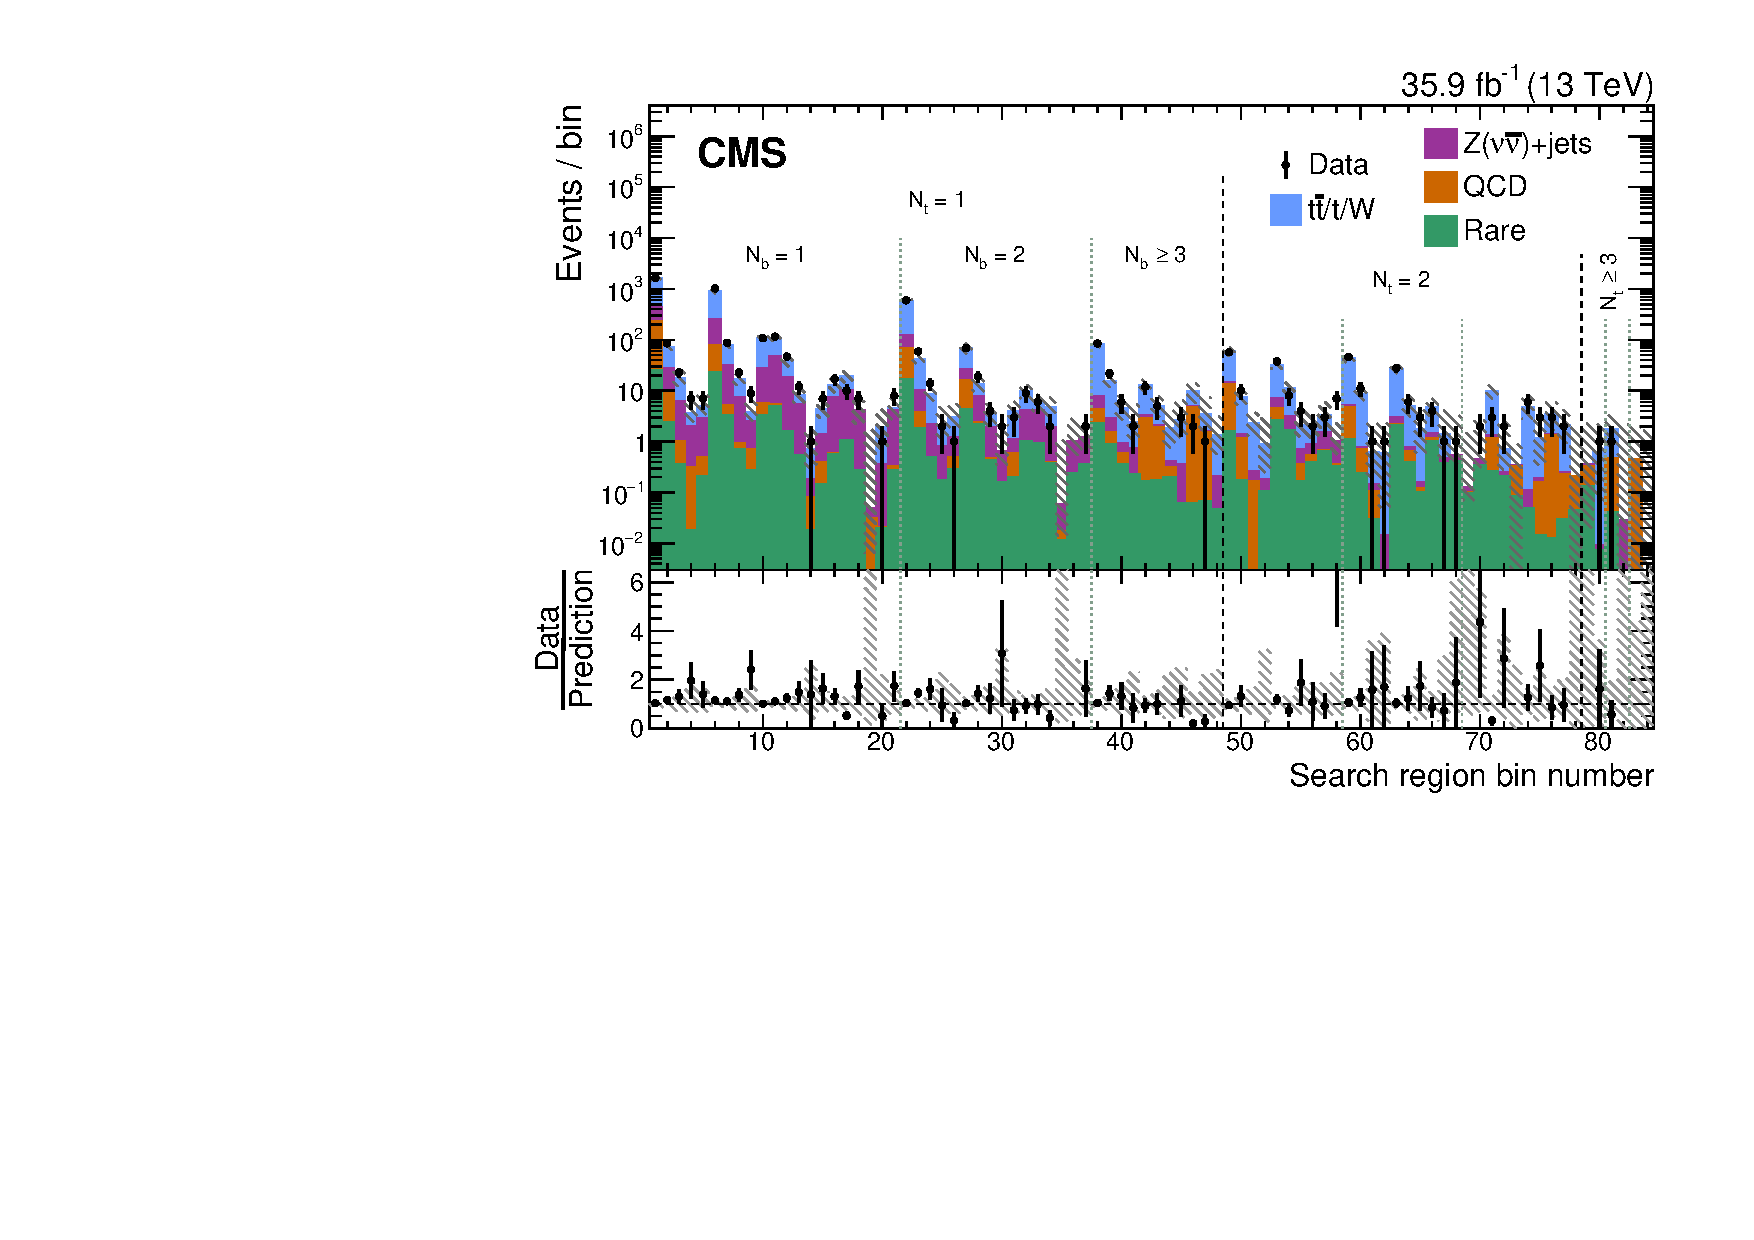
\includegraphics[width=0.8\textwidth]{sections/mc4/Results/figures/UnblindPlots.pdf}
 \end{center}
 \caption{Observed event yields in data (black points) and predicted SM background (filled solid area) for the 84 search bins. The lower panel shows the ratio of data over total background prediction in each search bin. For both panels, the error bars show the statistical uncertainty associated with the observed data counts, and the grey (blue) hatched bands indicate the statistical (systematic) uncertainties in the total predicted background.}
 \label{fig:84sbunblind}
\end{figure}


\begin{figure}[ht!]
 \begin{centering}
  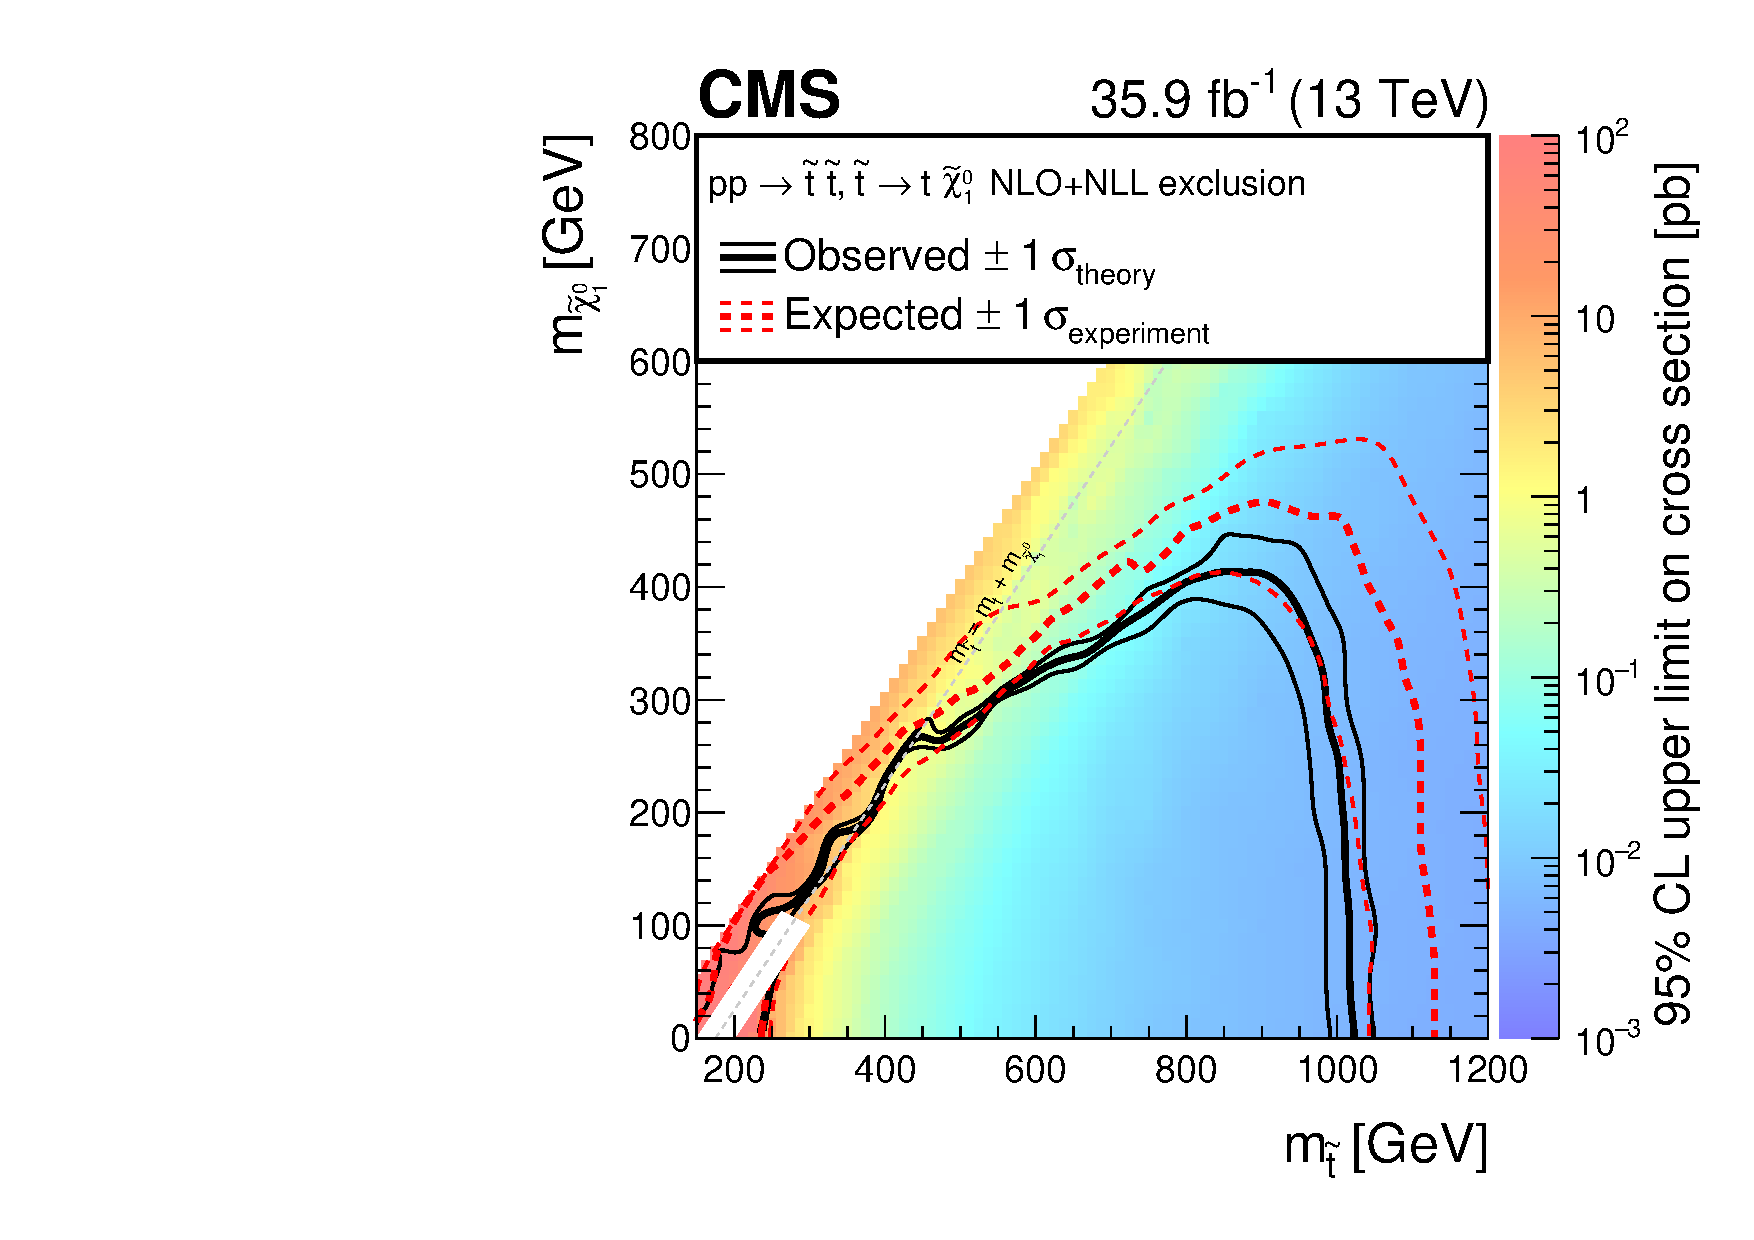
\includegraphics[width=0.50\textwidth]{sections/mc4/Results/figures/Covered_T2tt_OnlyXSEC.pdf}\\
  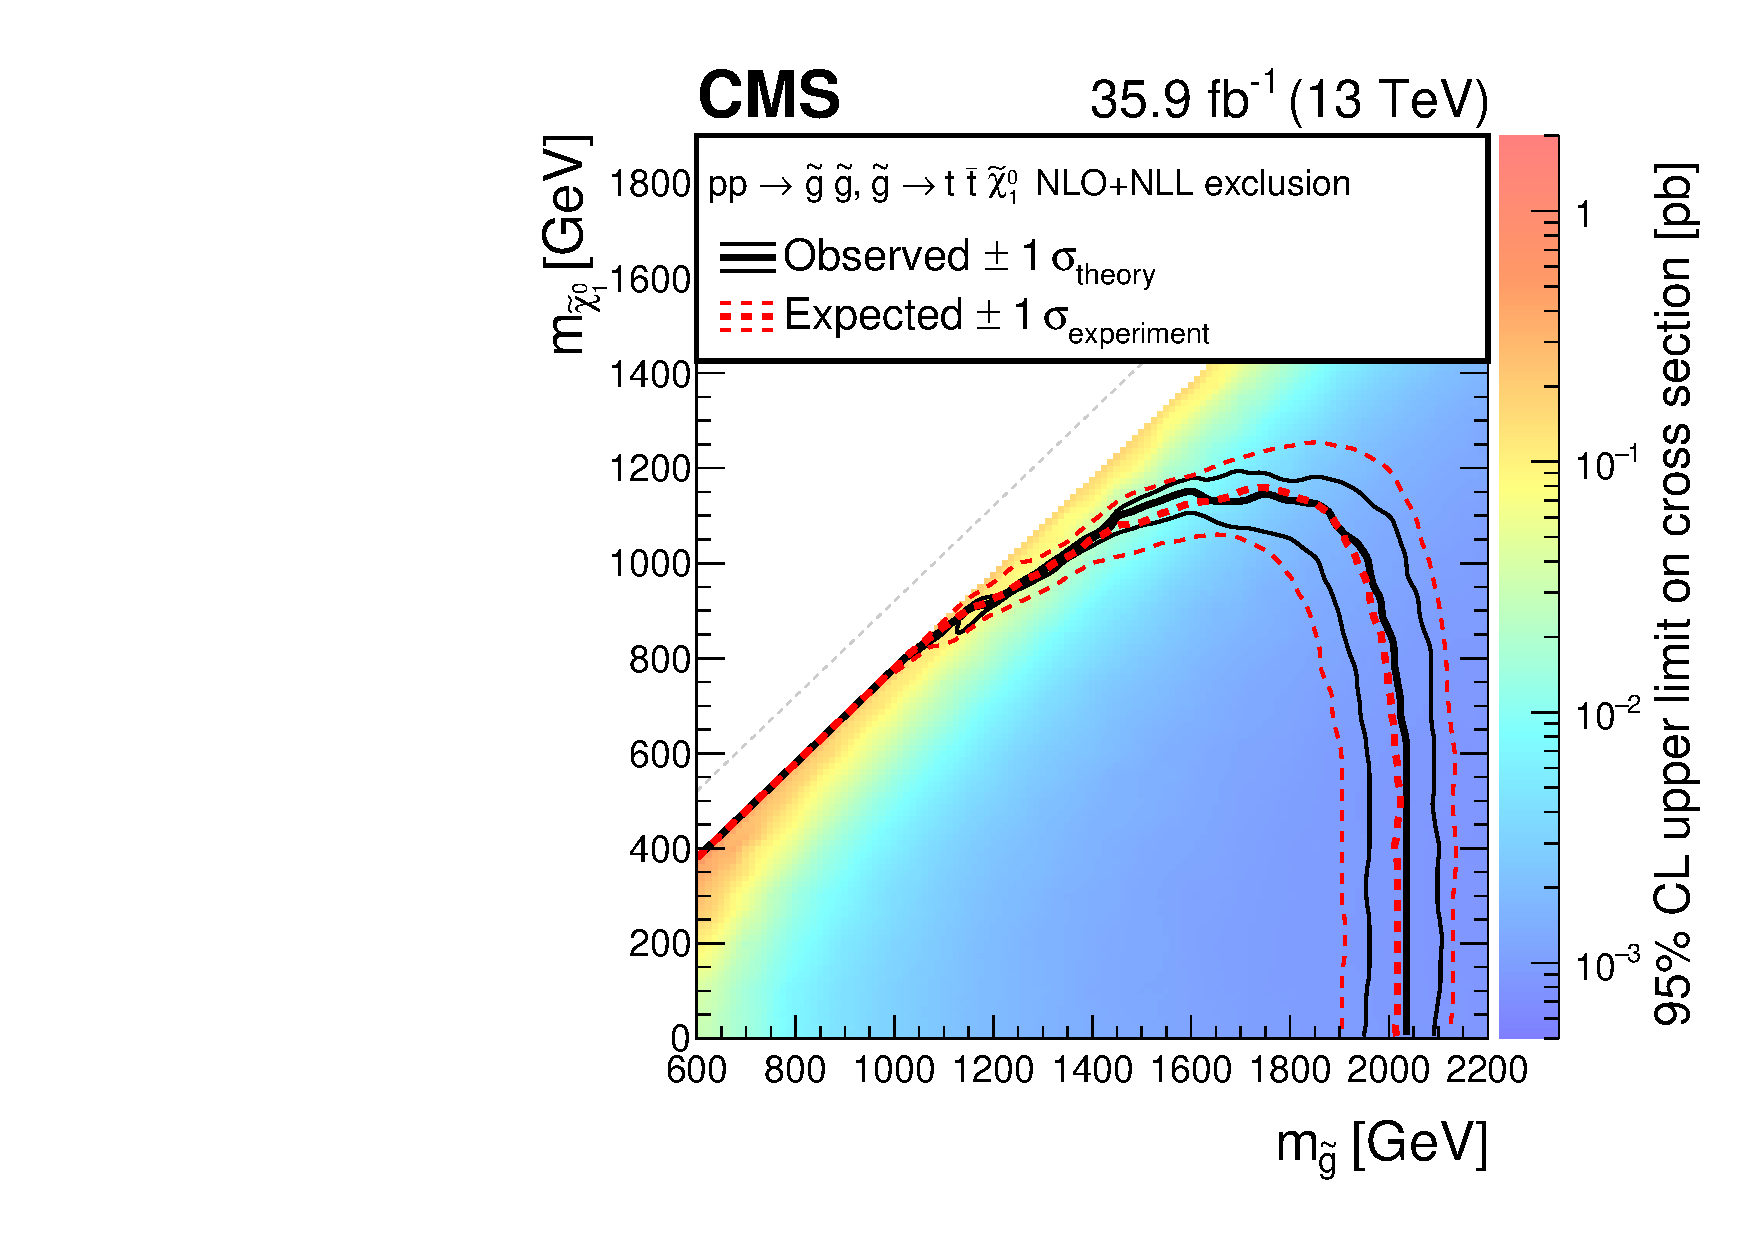
\includegraphics[width=0.40\textwidth]{sections/mc4/Results/figures/T1tttt_OnlyXSEC.pdf}
  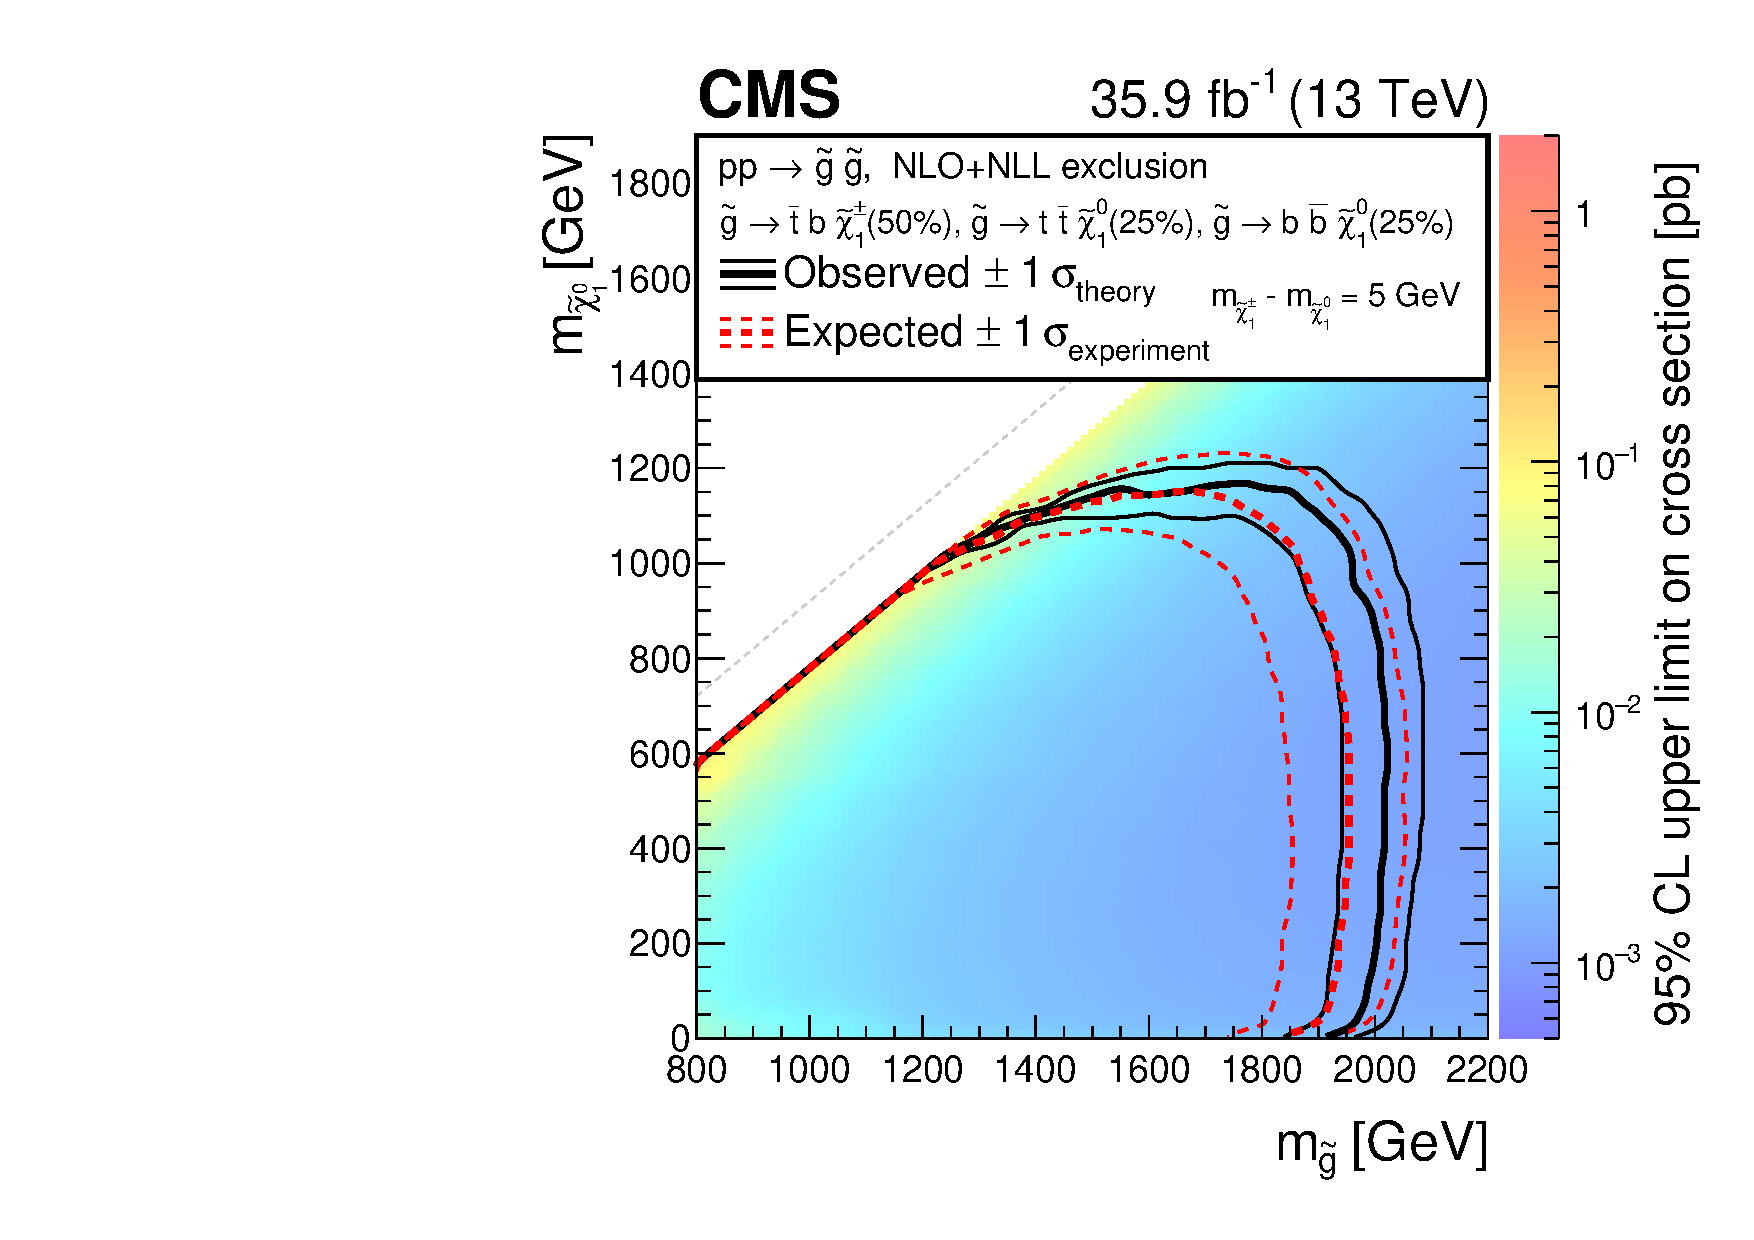
\includegraphics[width=0.40\textwidth]{sections/mc4/Results/figures/T1ttbb_OnlyXSEC.pdf}\\
  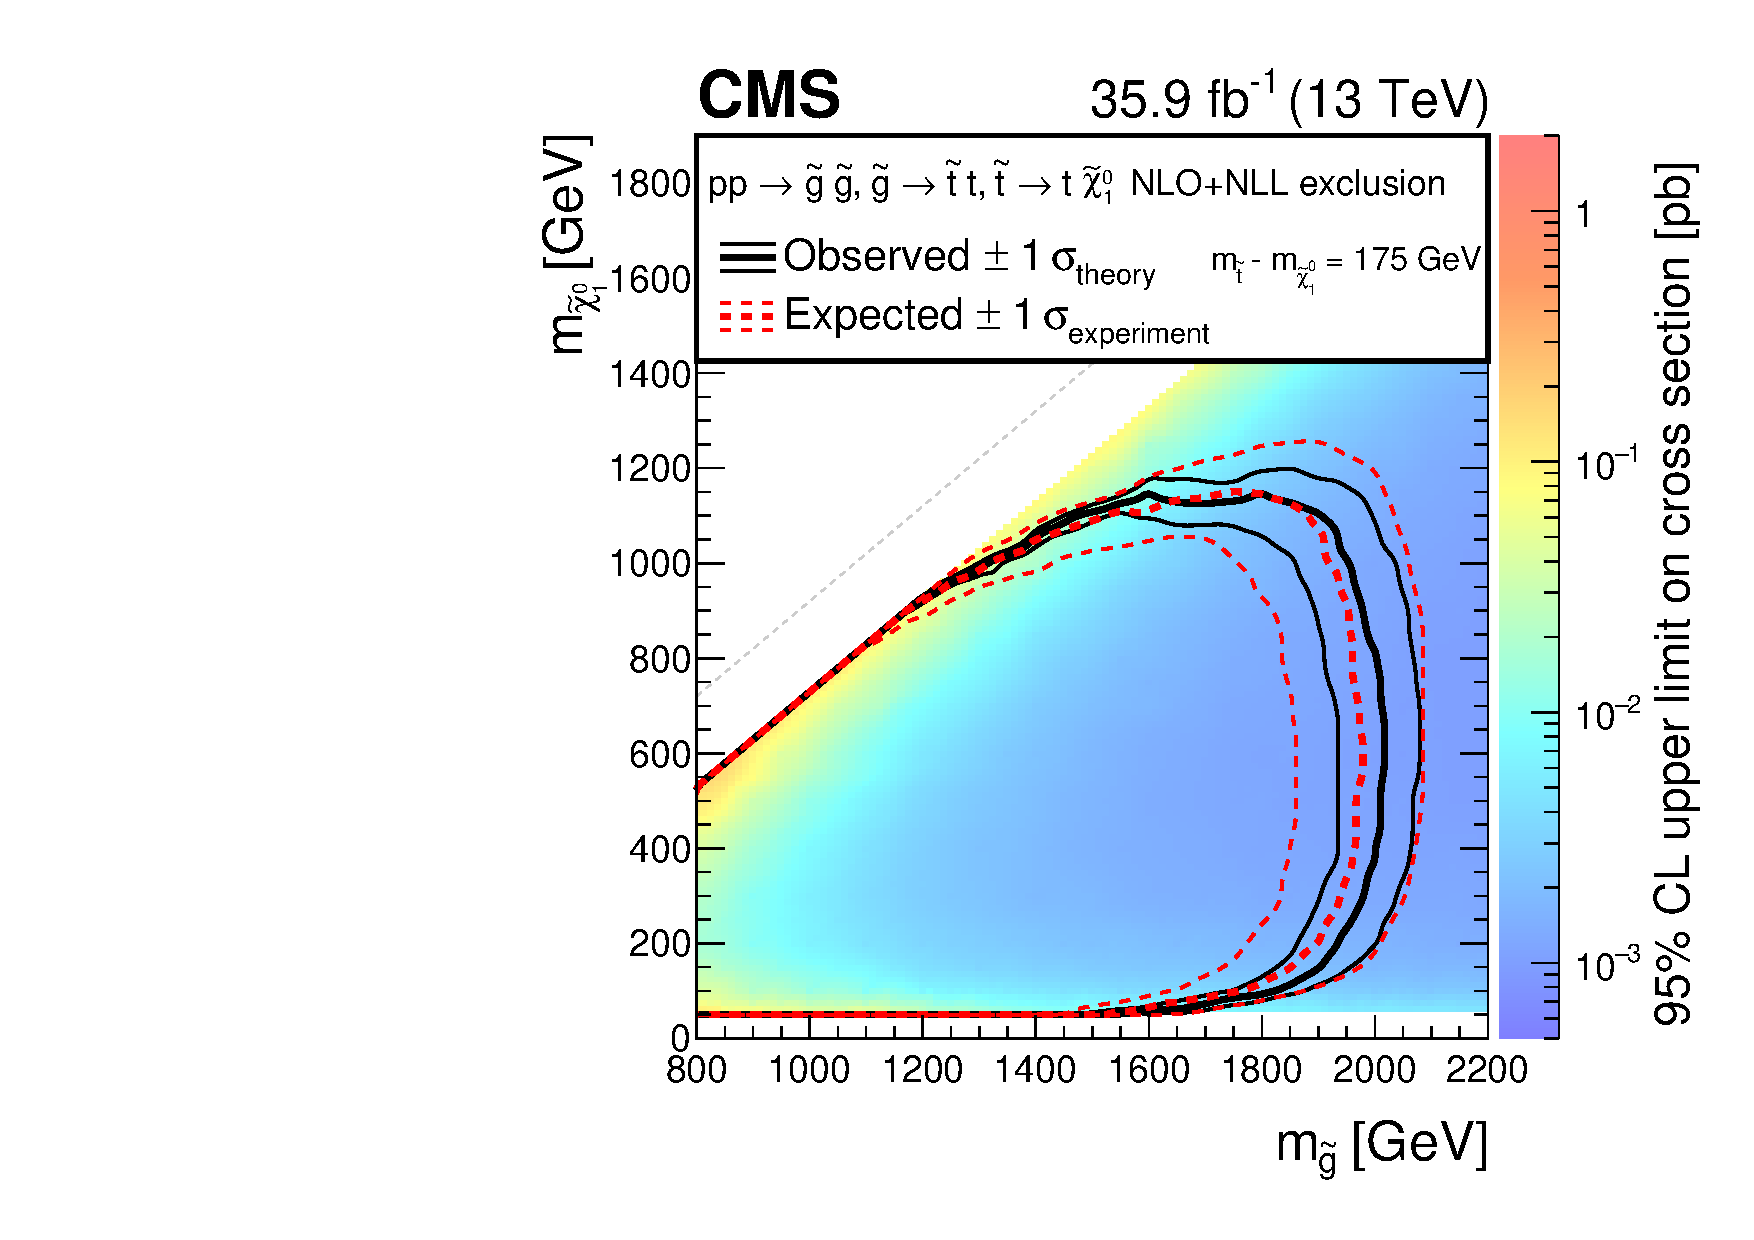
\includegraphics[width=0.40\textwidth]{sections/mc4/Results/figures/T5ttttdM175_OnlyXSEC.pdf}
  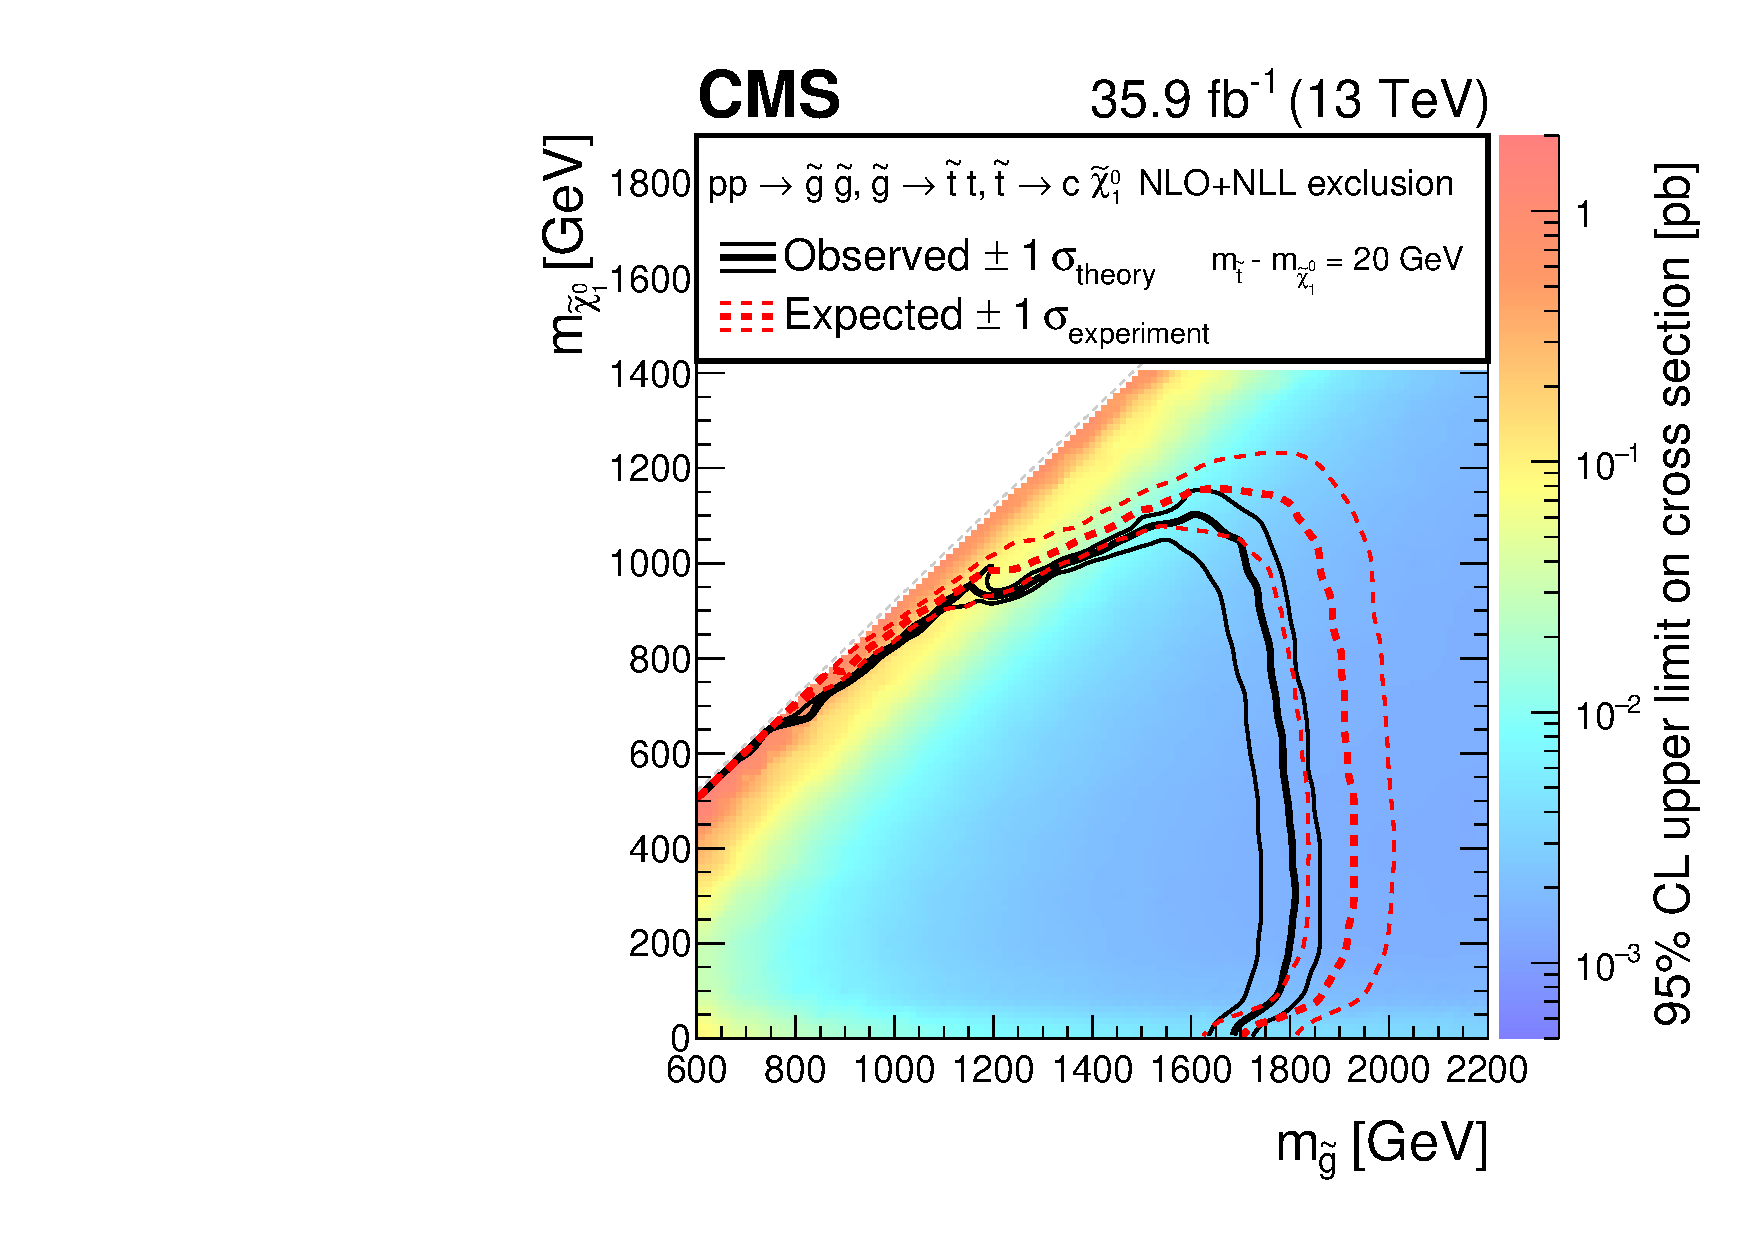
\includegraphics[width=0.40\textwidth]{sections/mc4/Results/figures/T5ttcc_OnlyXSEC.pdf}\\
  \caption{Exclusion limit at 95\% CL for the signal models in this search:
top squark pair production with the top squark decaying into a top quark and
neutralino (top),
and top squarks from cascade decays of gluinos (middle and bottom).
The SUSY simplified model topology shown at the top is referred to as T2tt,
the middle left model as T1tttt, middle right model as T1ttbb
the bottom left one as T5tttt and the bottom right one as T5ttcc.}
  \label{fig:signal_diagrams}
 \end{centering}
\end{figure}

